%!TEX program = xelatex
\documentclass[UTF8,a4paper,11pt]{article}
\usepackage[left=2.50cm, right=2.50cm, top=2.50cm,bottom=2.50cm]{geometry}
\geometry{a4paper}
%\usepackage[UTF8, heading = false, scheme = plain]{ctex}%格式
\usepackage{ctex}
%\usepackage{authblk} %添加机构,需要安装preprint包
\usepackage{graphicx} %添加图片
\usepackage{amsthm}
\usepackage{amsmath}
\renewcommand{\vec}[1]{\boldsymbol{#1}} % 生产粗体向量,而不是带箭头的向量
\usepackage{amssymb}
\usepackage{booktabs} % excel导出的大表格
\usepackage{amssymb}	%使用特殊的AMS符号
\usepackage{braket}	%狄拉克算符
\usepackage{cases} 
\usepackage{mathtools}  %左上下标
\usepackage{caption}
\usepackage{subfigure}
\usepackage{cite}
\usepackage{bm}   %加粗公式字体
\usepackage{enumitem}
\usepackage{hyperref}
\usepackage{tikz}
\usetikzlibrary{quantikz}
\hypersetup{colorlinks=true,linkcolor=black}	%去掉链接的红框
\usepackage[ruled,linesnumbered]{algorithm2e}  %添加算法伪码
%$\mathbb{R}$
%$\mathcal{R}$
%$\mathscr{R}$
%\newtheorem{definition}{Definition} %英文
%\newtheorem{theorem}{Theorem}
\newtheorem{definition}{定义} %中文
\newtheorem{lemma}{引理}
\newtheorem{theorem}{定理}
%\newenvironment{proof}{{\noindent\it 证明}\quad}{\hfill $\square$\par}


\title{常用数学笔记}
\author{Richard}
%\affil{***}
%date{2020年03月09日} %注释后显示为编译时日期

\begin{document}
\maketitle
\tableofcontents
\newpage
% 生成目录,请删除上面两行注释
%\listoffigures
%\newpage
% 生成图片列表,请删除上面两行注释

\section{代数}
在数学中,代数结构是指由一组元素和一些运算组成的数学对象。代数结构是数学中的一个重要概念,它涵盖了许多不同的数学概念,例如群、环、域、向量空间等。

代数结构的定义基于抽象的数学概念,它不依赖于元素的具体性质,而是关注元素之间的相互关系。因此,代数结构通常被描述为一组元素和一些运算,而不是一组具体的数值或对象。

代数结构的运算通常具有特定的性质,例如结合律、交换律、单位元素、逆元素等。这些性质使得代数结构成为一种有用的数学工具,可以用来研究各种数学问题,例如几何学、物理学、计算机科学等。
\subsection{集合}
\subsubsection{Support(支集或支撑集)}
The support of a real-valued function $f: X \rightarrow \mathbb{R}$, where $X$ is a set (often assumed to have some topological structure), is defined as the set of points in $X$ where $f$ is non-zero. Formally, this can be expressed as:

\[ \text{supp}(f) = \{ x \in X \mid f(x) \neq 0 \} \]

In the case where $X$ is a topological space, one typically takes the closure of this set:

\[ \text{supp}(f) = \overline{\{ x \in X \mid f(x) \neq 0 \}} \]

where $\overline{A}$ denotes the closure of the set $A$.

如果 $\text{supp}(f)$ 有界, 则称为紧支集. 将注意力从整个定义域转到函数值不为0(nontrivial)的点.

The support of a measure $\mu$ on a set $X$ (which is usually assumed to be a measurable space with a $\sigma$-algebra $\mathcal{F}$) is defined as the largest measurable set for which every measurable subset has positive measure. This can be expressed as:

\[ \text{supp}(\mu) = X \setminus \bigcup \{ A \in \mathcal{F} \mid \mu(A) = 0 \} \]

In the case where $X$ is a topological space, and the $\sigma$-algebra is the Borel $\sigma$-algebra (generated by the open sets), the support of the measure can also be defined in terms of open sets, as described in the previous message.

\subsection{群}
群(Group)是代数学中的一种基本概念,它是由一组元素和一个二元运算构成的代数结构。在群中,这个二元运算满足以下四个公理:
\begin{itemize}
\item 1. 封闭性:对于群中的任意两个元素 $a$ 和 $b$,它们的二元运算结果 $a * b$ 也必须属于这个群。
\item 2. 结合律:对于群中的任意三个元素 $a$、$b$ 和 $c$,它们的二元运算结果必须满足结合律,即 $(a * b) * c = a * (b * c)$。
\item 3. 单位元素:在群中,必须存在一个元素 $e$,使得对于群中的任意元素 $a$,它们的二元运算结果满足 $a * e = e * a = a$。
\item 4. 逆元素:对于群中的任意元素 $a$,必须存在一个元素 $a^{-1}$,使得它们的二元运算结果满足 $a * a^{-1} = a^{-1} * a = e$。

其中,$e$ 表示群中的单位元素,$a^{-1}$ 表示元素 $a$ 在群中的逆元素。
\end{itemize}
除了上述四个公理,群还具有一些基本性质,如下所示:
\begin{itemize}
\item 1. 群中的单位元素是唯一的。
\item 2. 群中的每个元素都有唯一的逆元素。
\item 3. 群中的二元运算满足消去律,即如果 $a * b = a * c$,那么 $b = c$。
\item 4. 群中的二元运算满足左右消去律,即如果 $a * b = c$,那么对于任意元素 $x$,都有 $b = a^{-1} * c$ 和 $a = c * b^{-1}$。
\item 5. 群中的二元运算满足对称律,即对于任意元素 $a$ 和 $b$,都有 $a * b = b * a$。
\item 6. 群中的二元运算满足单位元素的唯一性,即如果 $a * b = a$,那么 $b = e$。
\end{itemize}
一个典型的例子是整数加法群 $(\mathbb{Z}, +)$,其中 $\mathbb{Z}$ 表示整数集合,$+$ 表示加法运算。该群中的单位元素为 0,每个元素 $a$ 的逆元素为 $-a$,并且满足上述所有公理和性质。

另一个例子是旋转群 $(SO(3), \cdot)$,其中 $SO(3)$ 表示三维空间中的旋转矩阵集合,$\cdot$ 表示矩阵乘法。在该群中,单位元素是单位矩阵 $I$,每个旋转矩阵 $R$ 的逆元素是它的转置矩阵 $R^T$,并且满足上述所有公理和性质。

群论是代数学中的一个重要分支,它在数学、物理学、计算机科学等领域都有着广泛的应用。
\subsubsection{Lie群}
Lie群(Lie group)是一个同时具有群和微分流形结构的数学对象。具体来说,一个 Lie 群是一个群 $G$,同时也是一个实数域或复数域上的实流形或复流形,满足以下条件:

1. 群结构:$G$ 是一个群,即它有一个乘法运算 $\cdot$,满足结合律、单位元存在性和逆元存在性。

2. 流形结构:$G$ 是一个实数域或复数域上的实流形或复流形,即它可以用一族局部坐标系(local coordinate systems)覆盖,并且每个局部坐标系都与实数域或复数域上的欧几里得空间同胚(homeomorphic)。

3. 群运算是光滑的:乘法运算 $\cdot : G \times G \rightarrow G$ 和逆运算 $^{-1} : G \rightarrow G$ 都是光滑映射(smooth mappings)。

一个 Lie 群的微分结构使得我们可以在其上定义微分方程和微分几何问题,并且可以将 Lie 群的结构和性质与微分方程和微分几何联系起来。

典型的例子包括矩阵群(Matrix group),如一般线性群 $GL(n,\mathbb{R})$ 或 $GL(n,\mathbb{C})$,以及李群(Lie group)如旋转群 $SO(3)$ 和特殊线性群 $SL(n,\mathbb{R})$。

Lie 群是数学中的一个重要概念,它在数学、物理学、工程学等领域都有着广泛的应用。
\subsubsection{Poincaré群}
Poincaré群(Poincaré group)是时空对称性的数学表示,描述了物理学中的时空对称性。具体来说,Poincaré群是四维时空中的所有变换的群,包括时空平移、旋转和洛伦兹变换。在相对论物理学中,它是描述自由粒子运动的对称性群。

Poincaré群由四维时空中的时空平移生成元和洛伦兹变换生成元构成。其中时空平移生成元用四维矢量 $a=(a_0,a_1,a_2,a_3)$ 表示,其作用是将时空坐标 $x^\mu$ 变为 $x^\mu+a^\mu$。洛伦兹变换生成元包括三种类型:空间旋转、洛伦兹平移和洛伦兹变换。它们可以用四维反对称张量 $M^{\mu\nu}$ 表示,其作用是将时空坐标 $x^\mu$ 变为 $x^\mu+M^\mu_\nu x^\nu$。

因此,Poincaré群可以表示为所有时空坐标变换的集合,它的元素可以写成以下形式:

$$
\Lambda = \begin{pmatrix} \Lambda^0_0 & \Lambda^0_1 & \Lambda^0_2 & \Lambda^0_3 \\ \Lambda^1_0 & \Lambda^1_1 & \Lambda^1_2 & \Lambda^1_3 \\ \Lambda^2_0 & \Lambda^2_1 & \Lambda^2_2 & \Lambda^2_3 \\ \Lambda^3_0 & \Lambda^3_1 & \Lambda^3_2 & \Lambda^3_3 \end{pmatrix},
\quad
a = \begin{pmatrix} a^0 \\ a^1 \\ a^2 \\ a^3 \end{pmatrix},
$$

其中 $\Lambda$ 表示洛伦兹变换,$a$ 表示时空平移,它们满足以下限制:

1. $\Lambda$ 是一个 $4 \times 4$ 的矩阵,满足 $\det(\Lambda) = 1$。

2. $\Lambda$ 是一个洛伦兹变换,即它满足 $\Lambda^\mu_{\ \rho} \eta^{\rho\sigma} \Lambda^\nu_{\ \sigma} = \eta^{\mu\nu}$,其中 $\eta$ 是时空度规,$\eta^{\mu\nu}$ 是其逆矩阵。

3. $a$ 是一个四维矢量,即它满足 $a^\mu \in \mathbb{R}$。

Poincaré群的群乘法定义为:

$$
\Lambda_1 \cdot \Lambda_2 = \begin{pmatrix} \Lambda^0_1 \Lambda^0_2 - \Lambda^1_1 \Lambda^1_2 - \Lambda^2_1 \Lambda^2_2 - \Lambda^3_1 \Lambda^3_2 & \Lambda^0_1 \Lambda^0_2 - \Lambda^1_1 \Lambda^1_2 - \Lambda^2_1 \Lambda^2_2 - \Lambda^3_1 \Lambda^3_2 & \cdots & \Lambda^0_1 \Lambda^0_2 - \Lambda^1_1 \Lambda^1_2 - \Lambda^2_1 \Lambda^2_2 - \Lambda^3_1 \Lambda^3_2 \\ \cdots & \cdots & \cdots & \cdots \\ \cdots & \cdots & \cdots & \cdots \\ \cdots & \cdots & \cdots & \Lambda^0_1 \Lambda^0_2 - \Lambda^1_1 \Lambda^1_2 - \Lambda^2_1 \Lambda^2_2 - \Lambda^3_1 \Lambda^3_2 \end{pmatrix},
$$

$$
a_1 \cdot a_2 = \begin{pmatrix} a^0_1 + a^0_2 \\ a^1_1 + a^1_2 \\ a^2_1 + a^2_2 \\ a^3_1 + a^3_2 \end{pmatrix},
$$

其中 $\cdot$ 表示矩阵乘法和矢量加法。

Poincaré群是物理学中非常重要的一个概念,它在狭义相对论、量子场论、高能物理等领域都有广泛的应用。

\subsubsection{Lorentz群}
Lorentz群(Lorentz group)是指四维时空中的洛伦兹变换所组成的群,其中洛伦兹变换是指四维时空中的线性变换,保持时空间隔不变的变换。洛伦兹群是相对论中的对称性群,描述了相对论中的时空对称性。

具体来说,洛伦兹群包括两个部分:旋转群(rotation group)和洛伦兹平移群(Lorentz boost)。旋转群是三维空间旋转的群,洛伦兹平移群是指在四维时空中的时间和空间的平移。这两个部分可以组合成洛伦兹变换,表示为一个 $4\times4$ 的矩阵:

$$
\Lambda = \begin{pmatrix} \Lambda^0_0 & \Lambda^0_1 & \Lambda^0_2 & \Lambda^0_3 \\ \Lambda^1_0 & \Lambda^1_1 & \Lambda^1_2 & \Lambda^1_3 \\ \Lambda^2_0 & \Lambda^2_1 & \Lambda^2_2 & \Lambda^2_3 \\ \Lambda^3_0 & \Lambda^3_1 & \Lambda^3_2 & \Lambda^3_3 \end{pmatrix},
$$

其中 $\Lambda^{\mu\nu}$ 表示变换矩阵的元素。洛伦兹群的元素必须满足以下条件:

1. $\Lambda$ 是一个 $4\times4$ 的正交矩阵,即 $\Lambda^T \eta \Lambda = \eta$,其中 $\eta$ 是时空度规矩阵,具体来说,$\eta = \text{diag}(1,-1,-1,-1)$。

2. $\Lambda$ 的行列式为 $+1$ 或 $-1$,即 $\det(\Lambda) = \pm 1$。

洛伦兹群可以分为两个部分,分别是 proper Lorentz群和 improper Lorentz群。proper Lorentz群指的是行列式为 $+1$ 的洛伦兹变换,它包括三维旋转和洛伦兹变换。improper Lorentz群指的是行列式为 $-1$ 的洛伦兹变换,它包括时间反演变换和空间反演变换。

Lorentz群是相对论中非常重要的一个概念,它在狭义相对论、量子场论、高能物理等领域都有广泛的应用。

\subsubsection{Clifford群}
Clifford群(Clifford group)是一个与 Clifford 代数相关的群。Clifford 代数是由矢量空间 $V$ 和一个对称双线性型 $\langle \cdot, \cdot \rangle : V \times V \rightarrow \mathbb{C}$ 生成的代数。Clifford 群是由 Clifford 代数的自同构群给出的,即保持 Clifford 代数结构不变的线性变换组成的群。

具体来说,设 $V$ 是一个 $n$ 维实矢量空间,$\{e_1, e_2, \ldots, e_n\}$ 是它的一组基。定义 Clifford 代数 $\text{Cl}(V,\langle \cdot,\cdot \rangle)$ 是在 $\{e_1, e_2, \ldots, e_n\}$ 基下由以下元素生成的代数:

1. $e_1, e_2, \ldots, e_n$,它们满足 $e_i^2 = \langle e_i, e_i \rangle$。

2. $e_ie_j + e_je_i$,其中 $i \neq j$。

3. $1$,它是单位元。

Clifford 群 $\text{Cliff}(V,\langle \cdot,\cdot \rangle)$ 是由 Clifford 代数的自同构群给出的,即保持 Clifford 代数结构不变的线性变换组成的群。具体来说,Clifford 群是由以下元素生成的群:

1. $\pm 1$,其中 $1$ 是单位元。

2. $v$,其中 $v$ 是 $V$ 中的任意一个非零向量。

3. $uvu^{-1}$,其中 $u$ 是 Clifford 群中的任意一个元素,$v$ 是 $V$ 中的任意一个非零向量,满足 $\langle v,v\rangle = 1$。

Clifford 群在量子信息理论和量子计算中具有重要的作用,例如在量子纠缠和量子误差纠正中的应用。

\subsubsection{辛群}
辛群(Symplectic Group)是一个重要的数学概念,在数学、物理学和工程学等领域中都有广泛的应用。定义:

设 $V$ 是一个 $2n$ 维实向量空间,$J$ 是一个 $2n\times 2n$ 的矩阵,满足以下条件:
\begin{itemize}
\item $J$ 是反对称的,即 $J^T = -J$;
\item $J$ 是非退化的,即 $\det(J) \neq 0$。
\end{itemize}
辛群 $\operatorname{Sp}(n)$ 是由 $n\times n$ 的实矩阵 $A$ 所组成的群,满足以下条件:

$$A^TJA = J,$$

其中 $J$ 是上面定义的矩阵。

性质:
\begin{itemize}
\item 辛群 $\operatorname{Sp}(n)$ 是一个非交换的李群,它的维数为 $n(2n+1)$。
\item 辛群 $\operatorname{Sp}(n)$ 的子群包括正交群 $\operatorname{O}(2n)$、特殊正交群 $\operatorname{SO}(2n)$、辛向量群 $\operatorname{Sp}(2n,\mathbb{R})$ 和辛矩阵群 $\operatorname{Sp}(2n,\mathbb{Z})$。
\item 辛群 $\operatorname{Sp}(n)$ 的李代数是由 $n\times n$ 的反对称实矩阵构成的矩阵代数 $\mathfrak{sp}(n)$,它的维数为 $n(2n-1)$。
\item 辛群 $\operatorname{Sp}(n)$ 是保辛变换的群,即它保持辛结构不变,因此在物理学中经常用于描述哈密顿系统的对称性,也在工程学中应用于控制系统设计和机器人学等领域。
\end{itemize}

应用:

辛群在数学、物理学和工程学等领域中都有广泛的应用。其中,量子力学和哈密顿力学中的辛结构、辛变换和辛群都是基础概念。在控制系统设计、机器人学和信号处理等领域中,辛群也有重要的应用。

具体来说,辛群在量子力学中用于描述系统的辛结构、辛变换和辛群,它们可以用于描述量子比特的演化、量子态的变换和量子系统的纠缠等问题。在控制系统设计和机器人学中,辛群可以用于描述系统的对称性,从而帮助设计控制算法和构造机器人模型。在信号处理中,辛群可以用于构造正交小波等信号分析工具。

\subsection{环}
环(Ring)是由一组元素和两个二元运算(加法和乘法)组成的代数结构。在环中,加法和乘法运算必须满足以下公理:
\begin{itemize}
\item 1. 加法运算构成一个阿贝尔群,即满足封闭性、结合律、交换律、单位元素和逆元素等性质。
\item 2. 乘法运算满足封闭性和结合律。
\item 3. 乘法运算对加法运算满足分配律。
\end{itemize}
环中的元素通常记作 $R$,加法运算记作 $+$,乘法运算记作 $\cdot$。通常会省略乘法运算的符号,即 $a \cdot b$ 简写为 $ab$。环可以是有限的或无限的,可以是交换环(即乘法满足交换律)或非交换环。

下面是一些环的性质:
\begin{itemize}
\item 1. 环中的加法单位元素是唯一的,通常记作 $0$。
\item 2. 环中的乘法单位元素是唯一的,通常记作 $1$。
\item 3. 环中的元素可能没有逆元素,即使有逆元素也不一定唯一。
\item 4. 环中乘法的左分配律和右分配律是等价的。
\item 5. 如果存在一个元素 $a$,使得 $ab = ac$,那么在一些条件下可以从等式两边消去 $a$,即 $b = c$。
\item 6. 如果环 $R$ 是交换环,则环 $R$ 中的每个非零元素都有唯一的逆元素。
\end{itemize}
一个典型的例子是整数环 $(\mathbb{Z}, +, \cdot)$,其中 $\mathbb{Z}$ 表示整数集合,$+$ 表示加法运算,$\cdot$ 表示乘法运算。在该环中,加法运算和乘法运算满足上述所有公理和性质。

另一个例子是多项式环 $(F[x], +, \cdot)$,其中 $F$ 是一个域,$x$ 是一个形式变量,$F[x]$ 表示所有以 $x$ 为变量、系数在 $F$ 中的多项式的集合。在该环中,加法运算和乘法运算分别定义为多项式的加法和乘法运算,满足上述所有公理和性质。

环论是代数学中的一个重要分支,它在代数、数论、几何、物理学等领域都有着广泛的应用。



\subsection{域}
域(Field)是一种包含加、减、乘、除四种基本运算的代数结构,具有以下性质:
\begin{itemize}
\item 1. 加法和乘法都是可交换的:对于任意 $a,b \in F$,有 $a+b=b+a$ 和 $ab=ba$。
\item 2. 加法和乘法都是可结合的:对于任意 $a,b,c \in F$,有 $(a+b)+c=a+(b+c)$ 和 $(ab)c=a(bc)$。
\item 3. 加法和乘法都有唯一的单位元素:加法单位元素通常表示为 $0$,乘法单位元素通常表示为 $1$。对于任意 $a \in F$,有 $a+0=a$ 和 $a\cdot 1=a$。
\item 4. 每个非零元素都有唯一的逆元素:对于任意 $a \neq 0$,存在一个唯一的元素 $a^{-1}$,使得 $aa^{-1}=a^{-1}a=1$。
\item 5. 加法和乘法满足分配律:对于任意 $a,b,c \in F$,有 $a(b+c)=ab+ac$。
\item 6. 零元素和单位元素不相等:$0 \neq 1$。
\end{itemize}
一个典型的例子是实数域 $(\mathbb{R},+,\cdot)$,其中 $\mathbb{R}$ 表示实数集合,$+$ 表示加法运算,$\cdot$ 表示乘法运算。在该域中,加法和乘法满足上述所有公理和性质。

另一个例子是有理数域 $(\mathbb{Q},+,\cdot)$,其中 $\mathbb{Q}$ 表示有理数集合,$+$ 表示加法运算,$\cdot$ 表示乘法运算。在该域中,加法和乘法满足上述所有公理和性质。

域论是代数学中的一个重要分支,它在代数、数论、几何、物理学等领域都有着广泛的应用。

\subsection{代数}
\begin{definition}[Algebra]
An algebra $\mathcal{A}$ over a field $F$ is a nonempty set $\mathcal{A}$, together with three operations, called addition (denoted by $+$), multiplication (denoted by juxtaposition) and scalar multiplication (also denoted by juxtaposition), for which the following properties hold:
\begin{itemize}
\item $\mathcal{A}$ is a vector space over $F$ under addition and scalar multiplication.
\item $\mathcal{A}$ is a ring under addition and multiplication.
\item If $r\in F$ and $a,b\in \mathcal{A}$, then 
$$r(ab)=(ra)b=a(rb)$$
\end{itemize}
Thus, an algebra is a vector space in which we can take the product of vectors, or a ring in which we can multiply each element by a scalar (subject, of course, to additional requirements as given in the definition).
\end{definition}
\begin{figure}[htb!]
\centering
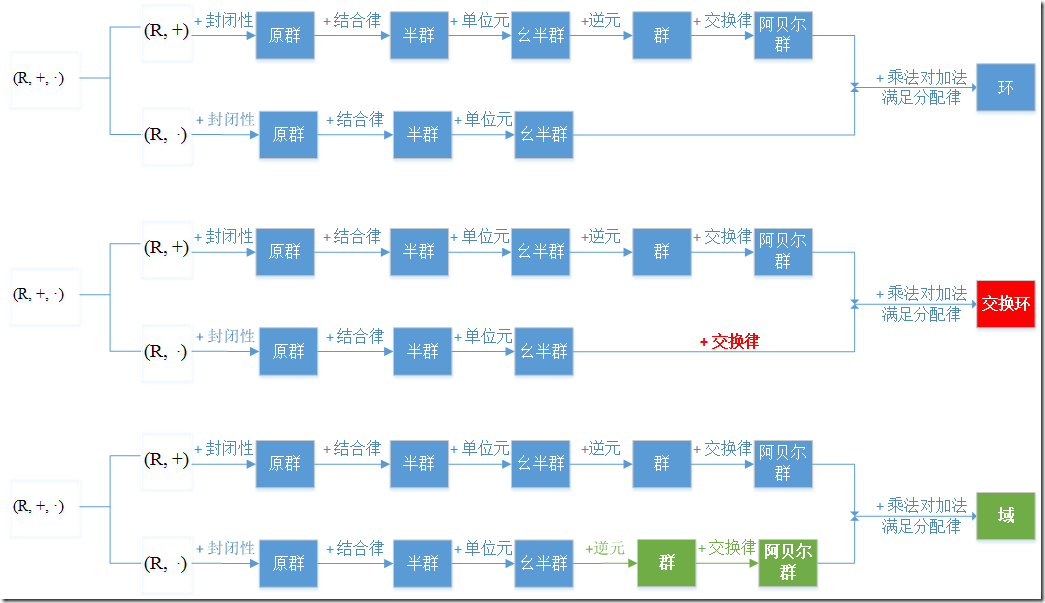
\includegraphics[width=0.8\textwidth]{figure/algebra.png}  
\caption{各类空间以及对应关系.}
\label{fig:space}
\end{figure}

\subsubsection{Clifford代数}
Clifford代数是一种重要的数学结构,它在数学、物理学、计算机科学等领域中都有广泛的应用。它是由 William Kingdon Clifford 在19世纪提出的,用于研究多元向量空间上的代数结构。定义:

设 $V$ 是一个 $n$ 维实向量空间,$q: V \rightarrow \mathbb{R}$ 是一个二次型,即:

$$
q(v) = \sum_{i=1}^n\sum_{j=1}^na_{ij}v_iv_j,
$$

其中 $a_{ij} \in \mathbb{R}$ 是常数,$v = (v_1, v_2, \ldots, v_n) \in V$。

Clifford代数 $C\ell_{p,q}$ 是由 $p$ 个生成元 $\{e_1, e_2, \ldots, e_p\}$ 和 $q$ 个生成元 $\{f_1, f_2, \ldots, f_q\}$ 所生成的代数,满足以下关系:
\begin{itemize}
\item $e_i^2 = 1$,$f_j^2 = -1$,$i=1,2,\ldots,p$,$j=1,2,\ldots,q$;
\item $e_ie_j = -e_je_i$,$f_if_j = -f_jf_i$,$i\neq j$;
\item $e_if_j = -f_je_i$,$i=1,2,\ldots,p$,$j=1,2,\ldots,q$;
\item $e_1e_2\cdots e_p f_1f_2\cdots f_q = (-1)^{pq}f_1f_2\cdots f_q e_1e_2\cdots e_p$。
\end{itemize}
其中第4个关系是对于 $p+q$ 为奇数时的情形,如果 $p+q$ 为偶数,则该关系可以简化为 $e_1e_2\cdots e_p f_1f_2\cdots f_q = f_1f_2\cdots f_q e_1e_2\cdots e_p$。

性质:
\begin{itemize}
\item Clifford代数 $C\ell_{p,q}$ 是一个关于 $\mathbb{R}$ 的 $2^{p+q}$ 维代数,它是一个实的、非交换的、非结合的代数。
\item Clifford代数 $C\ell_{p,q}$ 中的元素可以看作 $n=p+q$ 维实向量空间中的多元向量,其中每个生成元对应一个向量的坐标。
\item Clifford代数 $C\ell_{p,q}$ 中的元素可以表示为 $2^p \times 2^q$ 个矩阵的线性组合,这些矩阵称为Clifford元素。
\end{itemize}

Clifford代数在物理学、计算机科学、数学等领域中都有广泛的应用。其中,量子计算中的Clifford门和量子误差校正都使用了Clifford代数。

具体来说,量子计算中的Clifford门是一种重要的门操作,可以用来实现量子态的制备、量子态的测量、量子纠缠等操作。同时,量子误差校正中的Clifford代数可以用来描述量子比特的误差,并且可以用来构造保护量子比特的量子码。
\subsubsection{辛代数}
辛代数(Symplectic Algebra)是一个重要的数学概念,在数学、物理学和工程学等领域中都有广泛的应用。它是由辛向量空间上的反对称双线性形式构成的矩阵代数,包含了辛变换的所有信息。定义:

设 $(V,\omega)$ 是一个 $2n$ 维实向量空间,$\omega$ 是一个反对称双线性形式,即 $\omega(v,w) = -\omega(w,v)$。辛代数 $\mathfrak{sp}(V,\omega)$ 是由 $2n\times 2n$ 的矩阵 $A$ 所组成的矩阵代数,满足以下条件:

1. $A$ 是反对称的,即 $A^T = -A$;
2. $A$ 满足以下Jacobi恒等式(Jacobi identity):

$$
[A,[A,B]] + [B,[B,A]] = 0,
$$

其中 $[A,B] = AB - BA$ 是矩阵的对易子。

性质:

1. 辛代数 $\mathfrak{sp}(V,\omega)$ 是一个Lie代数,即它是一个满足Jacobi恒等式的矩阵代数。

2. 辛代数 $\mathfrak{sp}(V,\omega)$ 的维数为 $n(2n+1)$。

3. 辛代数 $\mathfrak{sp}(V,\omega)$ 中的元素可以表示为 $2n\times 2n$ 的反对称矩阵,它们是辛群的李代数。

4. 辛代数 $\mathfrak{sp}(V,\omega)$ 是保辛变换的代数.

\end{document}
